\documentclass[12pt]{article}
\usepackage{a4wide}
\usepackage{glossaries}
\usepackage{hyperref}
\usepackage{tikz}
\usetikzlibrary{calc,trees,positioning,arrows,chains,shapes.geometric,%
    decorations.pathreplacing,decorations.pathmorphing,shapes,%
    matrix,shapes.symbols}
\tikzset{
>=stealth',
  bbox/.style={
    rectangle, 
    rounded corners, 
    % fill=black!10,
    draw=black, very thick,
    text width=10em, 
    minimum height=2em, 
    text centered}, 
    %on chain},
  ybox/.style={
    rectangle, 
    rounded corners, 
    % fill=black!10,
    draw=black, very thick,
    text width=10em, 
    minimum height=2em, 
    minimum width=40em,
    text centered}, 
    %on chain},
  line/.style={draw, thick, <-},
  element/.style={
    tape,
    top color=white,
    bottom color=blue!50!black!60!,
    minimum width=8em,
    draw=blue!40!black!90, very thick,
    text width=10em, 
    minimum height=3.5em, 
    text centered, 
    on chain},
  every join/.style={->, thick,shorten >=1pt},
  decoration={brace},
  tuborg/.style={decorate},
  tubnode/.style={midway, right=2pt},
}
\makeglossaries
 
\newglossaryentry{csc}
{
    name=CSC,
    description={Cooperative Storage Cloud}
}
 
\newglossaryentry{dht}
{
    name=DHT,
    description={Distributed Hash Table}
}

\newglossaryentry{p2p}
{
    name=P2P,
    description={Peer to Peer}
}

\newglossaryentry{uid}
{
    name=UID,
    description={User Identifier}
}

\newcommand{\al}{}
\newcommand{\ar}{}

\parindent 0pt
\parskip 6pt

\begin{document}

\tableofcontents
\clearpage

\section{Introduction and Description of the Work}

Making files available on the Internet is an important practical problem. It has applications ranging from simple file hosting to content synchronisation across multiple devices. The idea to think of the Internet as a storage medium rather than a communication platform lead to the concept of cloud storage. As the number of people owning multiple devices (computers, phones) and thus benefiting from cloud sync is growing, more and more companies are entering the business with their proprietary solutions. It is common for these systems to have a centralised entity and thus they inherit some problems:

\begin{itemize}
\item{scaling: $O(N)$ bandwidth resource required at the centre to distribute content to N users}
\item{single point of failure: if the central entity fails, the file becomes unavailable}
\item{privacy and ownership: the cloud provider has to be trusted with all the content which raises privacy and legal concerns especially if sensitive material is involved}
\end{itemize}

Peer-to-peer (P2P) file transfer protocols attempt to solve the performance problems by making use of the upload resources of each client. This allows in theory to distribute a file to N people in $O(\log N)$ time instead of $O(N)$.\footnote{Assuming a simplistic model of uniform link speeds, where in every timestep every peer in possession of the information duplicates it to another peer, thus doubling the number of peers that have the data.} Due to redundancy, these systems could also be more resilient to failure. In particular, if the system is completely decentralised there is no single point of failure.

However, they are often not completely decentralised. For example, it is common to use trackers for transfers using the Bittorrent protocol. These trackers are trusted parties responsible for tracking online users and information about the content they share. Since they are only communicating metadata, the scaling and resource requirement problems are not reached but the single point of failure remains. Distributed Hash Table (\gls{dht}) is a way to overcome the need for centralised peer discovery and bookkeeping. It is essentially a regular hash table maintained by a collection of peers, each having responsibility for storing and maintaining a part of the table.

There is a distinction between P2P file transfer protocols and storage clouds. The former is a way to send files on the Internet which requires at least one available peer in possession of the data. The latter creates an abstraction and provides a storage medium to the client. That it, users can perform upload and download operations on it. The way the content is structured and stored is abstracted away. For example, it may very well be the case that the content is dispersed over the underlying peers, each storing a portion of the data but none of them storing all of it. It turns out that such a scattered layout is actually beneficial both for the performance and availability of the system.

An important problem is caused by the transient nature of peers. They can connect and disconnect fairly rapidly without providing any guarantees. It is not only the bandwidth resources that disappear but also their local storage media with valuable information on them. P2P systems can use redundancy to attempt to provide a reliable and available storage platform on top of many unreliable peers.

\subsection{The project}
The aim of the project is to design and implement a cooperative storage cloud. This completely decentralised\footnote{Provided at least one available participating peer's IP address is known.} system would allow exchanging files between peers. Any peer would be able to publish its files which could be downloaded by other peers.


When sharing a file, after the initial upload phase the file will remain in the cloud. It will then be the cloud's responsibility to make the contents available to anyone. This means the owner of the file can log off, and so can any other peer. 

%The system has to be stable even in the face of continuous change of its peers. The required amount of replication has to be implemented to provide availability without much transfer overhead.


The underlying method of communication will be a Distributed Hash Table. Based on preliminary research, Chord's protocol seems appropriate for this use case. At the expense of the communication volume and the storage requirements scaling logarithmically with the number of peers, Chord offers invaluable promises relating to availability (discussed in 4.1).

\section{Resources Required}

I will use my own computer (Macbook Pro mid 2015) for this project. Both the source code and the dissertation will be tracked using git, which will be pushed to a repository in my Github account. In addition to this I will take daily backups of my work folder by syncing it to Dropbox, where I have over a terabyte of free space. My contingency plan for equipment failure is to use one of the MCS machines. To write my dissertation I will not use any packages not supported by \TeX live, which is installed on the MCS machines. Java development is also supported by the Eclipse IDE that I am familiar with. Any external libraries my project uses will be synced to Dropbox. Other than these, my project requires no special hardware or software and it would be relatively straightforward to continue with the work on an MCS machine.

The evaluation phase will require performance testing. I plan to use many MCS machines simultaneously with significant amount of local storage space on each (specifics to be determined in work block 2). The milestones address acquiring necessary permissions well in time.

\section{Starting Point}

I plan to write all code in Java. I do not have any experience with it other than that acquired through completing the practicals for the Object-Oriented Programming and Further Java courses, as well as my second year group project.

The relevant Tripos courses I have taken:
\begin{itemize}
\item{Object-Oriented Programming}
\item{Further Java}
\item{Computer Networking}
\item{Concurrent and Distributed Systems}
\item{Software and Interface Design}
\item{Software engineering}
\item{Security I}
\item{Algorithms}
\item{Operating Systems}
\end{itemize}

I have given a 20-minute talk about Bitcoin. The principles behind engineering this distributed currency will be relevant to designing my project.

I have completed an internship at Dropbox last summer. Dropbox is a company offering cloud storage. However, my work there was not relevant to this project.

Initial research has been conducted about peer-to-peer protocols as part of writing the proposal and designing the structure of my project.

\section{Substance and Structure of the Project}

The contents of this section are a result of preliminary planning and is subject to refinement during the initial planning and research phase of the project.

The front-end of the project will be a simple terminal application supporting the following:

\begin{itemize}
\item{Various information about the system state will be written to the terminal.}
\item{The user can enter commands to:}
\begin{itemize}
	\item{Retrieve a list of files stored for a user.}
	\item{Download a file from the list.}
	\item{Input a file name and upload the file.}

\end{itemize}
\end{itemize}

The back-end will be split into the following two main layers:

\begin{enumerate}
\item{Distributed Hash Table (\gls{dht})}
\item{Cooperative Storage Cloud (\gls{csc})}
\end{enumerate}

\vspace{0.5cm}

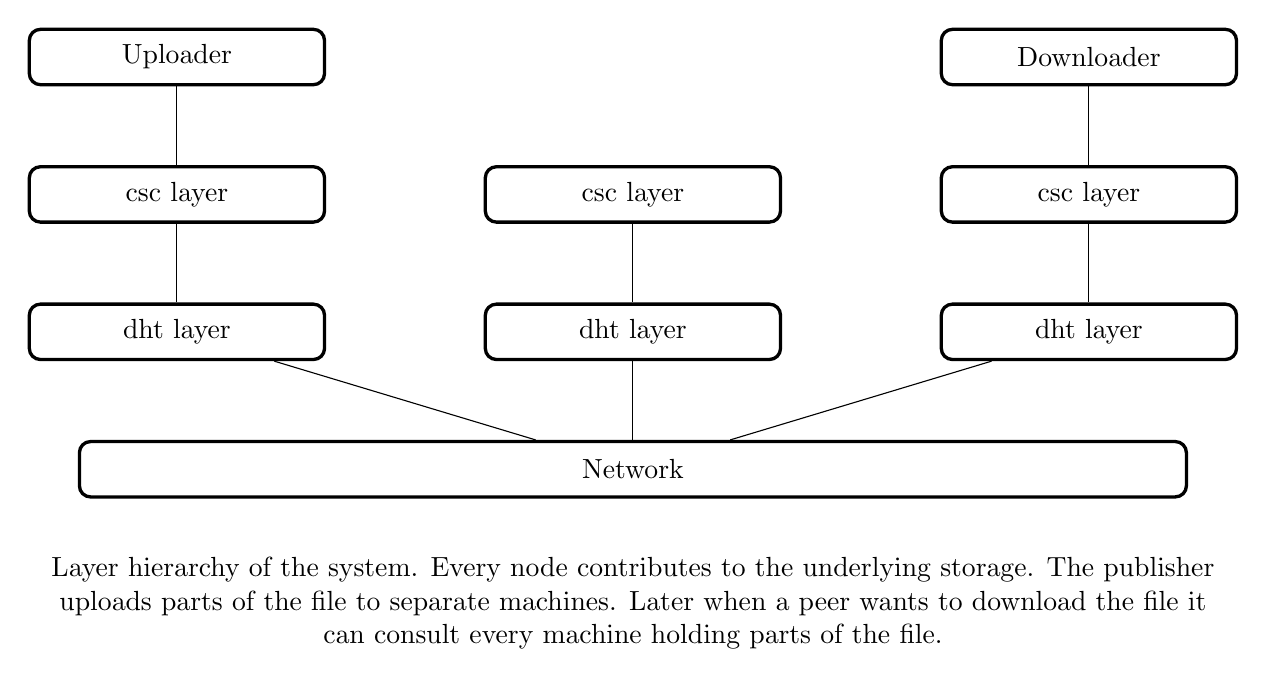
\begin{tikzpicture}[auto, node distance=2cm,>=latex']
        \tikzstyle{block} = [draw, rectangle];
        \tikzstyle{rblock}=[draw, shape=rectangle,rounded corners=0.5em];
        \node [bbox] (publisher) {Uploader};
        \node [bbox, below =1cm of publisher] (csc1) {\gls{csc} layer};
        \node [bbox, below =1cm of csc1] (dht1) {\gls{dht} layer};
        \node [bbox, right =2cm of csc1] (csc2) {\gls{csc} layer};
        \node [bbox, right =2cm of dht1, below =1cm of csc2] (dht2) {\gls{dht} layer};
        \node [bbox, right =2cm of csc2] (csc3) {\gls{csc} layer};
        \node [bbox, above =1cm of csc3] (downloader) {Downloader};
        \node [bbox, right =2cm of dht2, below =1cm of csc3] (dht3) {\gls{dht} layer};
        \node [ybox, below =1cm of dht2] (network) {Network};

        \node [below=1cm, align=flush center,text width=15cm] at (network)
        {
            Layer hierarchy of the system. Every node contributes to the underlying storage. The publisher uploads parts of the file to separate machines. Later when a peer wants to download the file it can consult every machine holding parts of the file.
        };
        %\node [block, below of=otsu] (gchannel) {Subtract the Green Channel};
        %\node [block, left of=gchannel] (closing) {Morphological Closing};

        \path[draw,-]
            (publisher) edge (csc1)
            (csc1) edge (dht1)

            (downloader) edge (csc3)
            (csc3) edge (dht3)

            (csc2) edge (dht2)

            (publisher) edge (csc1)
            (csc1) edge (dht1)

            %(otsu.east) -| (right) -- (left) |- (gchannel)
            (dht1) edge (network) 
            (dht2) edge (network) 
            (dht3) edge (network) 

            %(closing) edge (NN)
            %(NN) edge (limit)
            ;
\end{tikzpicture}

Additional layers such as cryptography, compression, diff analysis and file sync could be implemented on top of these as extensions. However to maximize utility, my focus will be skewed towards making the core layers more robust.

The core of the project will be designed relying on the following underlying assumptions:
\begin{enumerate}
\item{Connected peers do not have malicious intentions.}
\item{Peers are altruistic.}
\item{Hardware capabilities of connected peers are homogenous.}
\end{enumerate}

Dropping assumption 1 or 2 would make the protocol extremely hard to design. Dropping assumption 3 would lead to the introduction of virtual peers.\cite{dabekcfs}\cite{chord} It is a fairly straightforward but long implementation task to support them.

\subsection{Distributed Hash Table}
Implementing this layer as well as possible is high priority as it provides the core for the entire project. The layers above will not be able to provide better performance or availability characteristics than what this layer provides.

Desired characteristics are that with high probability:
\begin{itemize}
\item{Load balancing: for N nodes and K keys each node should be responsible for at most $\frac{(1+\epsilon)K}{N}$ keys, for $\epsilon=O(\log N)$.}
\item{The time to look up a value is $O(\log N)$.\footnote{even if the recent worload is systematic (eg. sequential) or random}.}
\item{Any node joining or leaving an N-node network will use $O(\log^2 N)$ messages to re-establish the routing invariants that the system relies on.}
\item{If every node fails with probability $\frac{1}{2}$, the system should still be able to serve lookups correctly in O(log N) time.}
\end{itemize}

Chord's \gls{dht} protocol satisfies all of the above. \cite{chord} An important property of the protocol is that it uses a consistent hashing function f. Each node is labelled $f(ip_{node})$ and stores all keys between its label and the next biggest label in the system. This guarantees that failures, even if they are related to each other (eg. power outage affecting all machines in Cambridge) will result in a random distribution of labels failing.

My plan is to implement Chord's protocol. There is some risk associated with me not being familiar with the scope of a practical implementation of the protocol. I will return to this during the research and planning phase of the project as a result of which slight changes to the protocol may be made. My emergency plan for the situation that even a basic implementation of Chord's protocol turns out to be infeasible, I will fall back to using an existing open-source implementation.\footnote{\url{https://github.com/netharis/Chord-Implementation}}\footnote{\url{http://sourceforge.net/projects/open-chord/}} None of these implementations are used widely, nor have I tested them since it is extremely unlikely that I will have to rely on them in this project.

\subsection{Cooperative Storage Cloud}

There are three layers of entities \gls{csc} stores in the \gls{dht}:
\begin{itemize}
\item{User level lookup: maps user identities (\gls{uid}) to filenames and file pointers}
\item{File level lookup: maps file pointers to block pointers and may provide additional metadata}
\item{Block level lookup: maps block pointers to block contents}
\end{itemize}

Pointers could be hash values so that data are randomly distributed across peers. This achieves load balancing and allows for simultaneous download of different chunks of the file from $N-1$ clients.

It is expected that each peer logged on has a different \gls{uid}. As a result, there will be no concurrent publish operations competing against each other by trying to upload files with the same filename. The publish operation will 

\begin{enumerate}
\item{Split the file into blocks of fixed size.}
\item{Upload these blocks keyed on the hash of each block to the block level lookup structure.}
\item{Upload the list of hashes to the file level lookup structure.}
\item{Upload the pointer to the file level lookup entry to the user level lookup structure.}
\end{enumerate}

If a node already stores a value for a key to be inserted, the operation of overwriting the old value has to be atomic. In this case eventual consistency is reached: it is possible that a download results in a slightly earlier (but consistent) version of the same file. However, as soon as the update reaches the file level lookup structure, the complete set of block pointers will be replaced.

An extension to this layer is changing replication: even though replication is handled in the underlying layer, the way it is handled is suboptimal. Copies of the blocks are distributed to some successors. However, using an Erasure Code algorithm such as Reed-Solomon would make it possible to provide the same availability with less redundancy.

\subsection{Implementation Method}

The project will be written in Java, not only because of it being cross-platform but also because it carries the least amount of risk: this is the language I am most familiar with, the quality of internal and third party libraries is outstanding, and so is the community support. I will use IntelliJ IDEA 14 or Eclipse as my IDE. These have built-in Git source control and testing features. For version control I will use Git and push upstream to my private Github repository. For writing unit tests I will use the JUnit library.


\section{Success Criteria}

Assuming that at least one IP address of the participating peers is known, the system should provide the following features to users without a centrally managed entity:

\begin{itemize}
\item{the contents of a file F can be uploaded}
\item{once the upload finishes and the system is stabilised, knowing the identity of the uploader any peer can download the contents of F}
\item{this remains true until F gets vacuumed, according to some vacuuming policy}
\end{itemize}

\section{Timetable and Milestones}

The project is split into two-week blocks, starting the day after the submission of the proposal. Blocks 1-11 are devoted to the project, blocks from 12 onwards are emergency slack. The plan is to use them mainly to revise for the written papers. If the project overruns, these blocks will be used to complete the core parts of the project but no extensions will be implemented during this time.


\subsection{Block 1: Chord's protocol}
\emph{24 Oct - 6 Nov}  % 1

During this work block I will deal with the highest risk parts of the project. This will primarily involve research into the Chord Distributed Hash Table protocol and the basics of Java's library support for networking. It is important to assess the scope of a practical implementation of Chord's protocol and devise a strategy for the implementation. Along with the research, an iterative approach of implementing the Chord layer will be started. This will initially focus on basic \gls{dht} functionality.

%Deliverables:
%\begin{itemize}
%\item{Unit tests.}
%\end{itemize}

Milestones:
\begin{itemize}
\item{Basic implementation of the \gls{dht} is complete, with the ability to store and retrieve entries but without any promises on performance and availability by EOD 4 Nov}
\end{itemize}


\subsection{Block 2: Additional research}
\emph{7 Nov - 20 Nov}  % 2

I will do more research into the elaborate aspects of Chord, eg. handling concurrent peer leaving or joining. Having gained more insight into Chord's protocol by this time, I will define the requirements and testing methods for the Chord module. The requirements will be split into necessary and desired properties.

Additional research will be conducted about how similar systems designed the file storage layer. I will focus in particular on Frank Davek's work on A Cooperative File System \cite{dabekcfs}. By the end of this block I will have written the preparaion chapter and designed the \gls{csc} layer. Consistent hashing algorithms will also be researched.

Milestones:
\begin{itemize}
\item{Plan for evaluation completed and submitted to my supervisor by EOD 17 Nov.}
\item{Preparation chapter completed and submitted for review to my supervisor by EOD 14 Nov.}
\item{Specification of my \gls{csc} protocol completed and submitted for review to my supervisor by EOD 19 Nov.}
\end{itemize}


\subsection{Block 3: Implementation}
\emph{21 Nov - 4 Dec}  % 3  | 4 Dec - Michaelmas ends

I will continue the implementation of Chord's protocol by iteratively extending the set of algorithms used with Chord's protocol to deliver the different performance/availability promises. By the end of this block, the implemented \gls{dht} layer will have all necessary properties defined in the previous block.

Milestones:
\begin{itemize}
\item{\gls{dht} layer is fully functional by EOD 2 Dec.}
\end{itemize}

\subsection{Block 4: Implementation}
\emph{5 Dec - 18 Dec}  % 4 | vacation

This block will be during the Christmas vacation. This means that I will have uninterrupted time to work on the project with two limitations: I will devote some time to spent with friends and family and I will have limited communication with my supervisor during this block. It makes sense to focus on parts that I can do with the least supervison. Therefore I will focus on implementing pre-defined components. I will prioritise on delivering a basic implementation of the \gls{csc} layer, having a decently working \gls{dht} layer in place. It will also address including the desired properties of Chord's protocol (defined in phase 2) to my implementation, to improve and finish the \gls{dht} layer.

Milestones:
\begin{itemize}
\item{Final version of the \gls{dht} completed by EOD 14 Dec.}
\item{\gls{dht} delivers the performance according to the pre-defined necessary promises, when tested locally by EOD 14 Dec.}
\item{A basic implementation of \gls{csc} complete, capable of storing the lists of published files per user by EOD 16 Dec.}
\end{itemize}

\subsection{Block 5: Implementation}
\emph{19 Dec - 1 Jan}  % 5  | vacation

Since both Christmas and New Years' Eve fall under this period of time, I will only plan one weeks' worth of work for this block. It will serve mainly as slack to absorb overruns without the whole project becoming late. Any remaining time will be used to work on the \gls{csc} layer.


Milestones:
\begin{itemize}
\item{Any milestone that was behind is done by EOD 30 Dec.}
\end{itemize}

\subsection{Block 6: Implementation and documentation}
\emph{2 Jan - 15 Jan}  % 6  | 12 Jan - Lent starts
I will finish the \gls{csc} layer. This will include using external libraries to perform consistent hashing and building the second and third level lookup layers. If the \gls{csc} layer is finished earlier than expected, I will use some of this time to implement extensions.

I will also write a draft implementation chapter of the dissertation during this block. This is intended to be an initial incomplete draft, to be improved in the next block. 

Lent term starts on the $12^{th}$ of Jan - I will reach out to the CL asking for permission to use the MCS machines for testing and evaluation in block 8.

Milestones:
\begin{itemize}
\item{\gls{csc} layer finished: files can be uploaded and downloaded without corruption by EOD 9 Jan}
\item{Draft implementation chapter written and submitted for review to my supervisor by EOD 13 Jan}
\end{itemize}

\subsection{Block 7: Testing and progress presentation}
\emph{16 Jan - 29 Jan} % 7  | 29 Jan - progress report deadline

During this block I will finish writing the implementation chapter of my dissertation.

Final integration tests will also be run and any problems that come up will be solved. Having tested each module extensively before it is expected that not many problems come up at a stage as late as this. I will also write the progress report during this block.

Milestones:
\begin{itemize}
\item{Implementation chapter written and submitted for review to my supervisor by EOD 27 Jan}
\item{Acquired permission to use MCS machines.}
\end{itemize}


\subsection{Block 8: Data Collection}
\emph{30 Jan - 12 Feb} % 8  

I will collect the required evaluation data during this block. The testing method for the \gls{dht} layer defined in block 2 will serve as the basis of what characteristics to test about the system. I will compare performance to other file transfer protocols, eg to BitTorrent Sync and FTP. MCS machines will likely be used for testing at scale, for which I will have acquired permission in the previous block. Collected data will be processed, graphs and figures will be generated.

Remaining time will be used as slack, or otherwise extensions will be implemented and corresponding changes will be documented in the dissertation.

Milestones:
\begin{itemize}
\item{Evaluation data collected by EOD 9 Feb.}
\item{Evaluation data processed by EOD 10 Feb.}
\end{itemize}

\subsection{Block 9: Evaluation}
\emph{13 Feb - 26 Feb} % 9

I will write the evaluation chapter during this block. All necessary data will have been collected in the previous block.

Milestones:
\begin{itemize}
\item{Evaluation chapter written and submitted for review to my supervisor by EOD 24 Feb.}

\end{itemize}

\subsection{Block 10: Conclusion}
\emph{27 Feb - 11 Mar} % 10 | 11 Mar Lent ends

The conclusion chapter and any supplementary material will be written during this block.

Milestones:
\begin{itemize}
\item{Conclusion chapter written and submitted for review to my supervisor by EOD 9 Mar.}

\end{itemize}

\subsection{Block 11: Editing}
\emph{12 Mar - 25 Mar} % 11

This block will be used as a slack time to finish writing the dissertation. Also, the coversheet, proforma and declaration of originality will be written during this block. Any spare time will be used for revision.

Milestones:
\begin{itemize}
\item{Dissertation printed and ready for submission by EOD 31 Mar.}
\end{itemize}

\subsection{Remaining blocks: Revision}
\emph{26 Mar - 15 May}  % 12 | emergency
%\emph{9 Apr - 22 Apr}  % 13 | 19 Apr - Easter starts
%\emph{23 Apr - 6 May}  % 14
%\emph{7 May - 15 May}  % 15 | May - deadline

These blocks will be used for revising for the written papers. My plan reflects that I prefer coagulating the time to spend on revision so that it is one bigger block close towards the exams. However, these blocks could also be used as emergency slack if necessary.

\clearpage
\begin{thebibliography}{9}

\bibitem{dabekcfs}
  Frank Dabek,
  \emph{A Cooperative File System},
  Massachusetts Institute of Technology,
  September 2001.

\bibitem{dabekdht}
  Frank Dabek,
  \emph{A Distributed Hash Table},
  Massachusetts Institute of Technology,
  September 2005.

\bibitem{chord}
  Ion Stoica, Robert Morris, David Karger, M. Frans Kaashoek, Hari Balakrishnan,
  \emph{Chord: A Scalable Peer-to-peer Lookup Service for Internet Applications},
  MIT Laboratory for Computer Science,
  2001.

\bibitem{bitdht}
  Andrew Loewenstern, Arvid Norberg,
  \emph{DHT Protocol},
  \url{http://www.bittorrent.org/beps/bep_0005.html}


\end{thebibliography}


\end{document}
